% ****** Start of file apssamp.tex ******
%
%   This file is part of the APS files in the REVTeX 4.1 distribution.
%   Version 4.1r of REVTeX, August 2010
%
%   Copyright (c) 2009, 2010 The American Physical Society.
%
%   See the REVTeX 4 README file for restrictions and more information.
%
% TeX'ing this file requires that you have AMS-LaTeX 2.0 installed
% as well as the rest of the prerequisites for REVTeX 4.1
%
% See the REVTeX 4 README file
% It also requires running BibTeX. The commands are as follows:
%
%  1)  latex apssamp.tex
%  2)  bibtex apssamp
%  3)  latex apssamp.tex
%  4)  latex apssamp.tex
%
\documentclass[%
 reprint,
%superscriptaddress,
%groupedaddress,
%unsortedaddress,
%runinaddress,
%frontmatterverbose, 
%preprint,
%showpacs,preprintnumbers,
%nofootinbib,
%nobibnotes,
%bibnotes,
 amsmath,amssymb,
 aps,
%pra,
%prb,
%rmp,
%prstab,
%prstper,
%floatfix,
]{revtex4-1}
%\usepackage{biblatex}
\usepackage{graphicx}% Include figure files
\usepackage{dcolumn}% Align table columns on decimal point
\usepackage{bm}% bold math
\usepackage{xspace}
\usepackage{float}
%\usepackage[showframe]{geometry}% http://ctan.org/pkg/geometry
\usepackage{lipsum}% http://ctan.org/pkg/lipsum
\usepackage[export]{adjustbox}
\usepackage{gensymb}
\usepackage{newunicodechar}
\usepackage[utf8]{inputenc}
\usepackage[table]{xcolor}
\usepackage{graphics}



 
%\usepackage{hyperref}% add hypertext capabilities
%\usepackage[mathlines]{lineno}% Enable numbering of text and display math
%\linenumbers\relax % Commence numbering lines

%\usepackage[showframe,%Uncomment any one of the following lines to test 
%%scale=0.7, marginratio={1:1, 2:3}, ignoreall,% default settings
%%text={7in,10in},centering,
%%margin=1.5in,
%%total={6.5in,8.75in}, top=1.2in, left=0.9in, includefoot,
%%height=10in,a5paper,hmargin={3cm,0.8in},
%]{geometry}

\begin{document}

%\preprint{APS/123-QED}
\newunicodechar{°}{\degree}
\newcommand {\gr}{$\gamma-ray$\xspace}
\newcommand {\grs}{$\gamma-rays$\xspace}
\newcommand {\gp}{$\gamma_{\text{photon}}$\xspace}
\newcommand {\cs}{$^{137}$Cesium \xspace}
\newcommand {\ba}{$^{133}$Barium \xspace}
\newcommand {\co}{$^{60}$Cobalt \xspace}
\newcommand {\na}{$^{22}$Sodium \xspace}
\title{Determining Electron Mass}% Force line breaks with \\


\author{Lee Allers, with Lucas Thoennes}
% \altaffiliation[Also at ]{Physics and Astronomy Department , University of New Mexico.}%Lines break automatically or can be forced with \\
%\affiliation{%
 %Authors' institution and/or address\\
 %This line break forced with \textbackslash\textbackslash
%}%


%\author{Charlie Author}
 %\homepage{http://www.Second.institution.edu/~Charlie.Author}
%\affiliation{
 %Second institution and/or address\\
 %This line break forced% with \\
%}%
%\affiliation{
 %Third institution, the second for Charlie Author
%}%
%\author{Delta Author}
%\affiliation{%
%Albuquerque, NM 87131\\
%1 University Blvd. \textbackslash\textbackslash
%}%

%\collaboration{CLEO Collaboration}%\noaffiliation

\date{\today}% It is always \today, today,
             %  but any date may be explicitly specified

\begin{abstract}
\begin{center} \textbf{Abstract}\end{center}
Using a \textit{NaI} scintillator detector and the Universal Computer spectrometer, we can measure the energy of gamma ray photons emitted by a radioactive source. This is because the scintillator detector functions by producing light\cite{S} when the gamma rays interact with the \textit{NaI} crystals. This is joined to a photomultiplier that converts the light into electrons. From the measured energies we interpret the data according to the Compton Scattering equation, \[\lambda ` - \lambda = \frac{h}{m_ec}(1 - cos\theta)\] where $\lambda$ is the initial wavelength, $\lambda `$ is the wavelength post-scattering, $h$ is the Planck constant, $m_e$ is the electron rest mass, $c$ is the speed of light, and $\theta$ is the scattered angle. From this data, we experimentally verify mass of the electron by analyzing the properties of the data, specifically, the Back Scatter peak, and Compton Edge produced by the incident photons and their energies on the scintillator detector.
%\begin{description}
%\item[Usage]
%Secondary publications and information retrieval purposes.
%\item[PACS numbers]
%May be entered using the \verb+\pacs{#1}+ command.
%\item[Structure]
%You may use the \texttt{description} environment to structure your abstract;
%use the optional argument of the \verb+\item+ command to give the category of each item. 
%\end{description}
\end{abstract}

%\pacs{Valid PACS appear here}% PACS, the Physics and Astronomy
                             % Classification Scheme.
%\keywords{Suggested keywords}%Use showkeys class option if keyword
                              %display desired
\maketitle

%\tableofcontents

\begin{figure}[ht!]
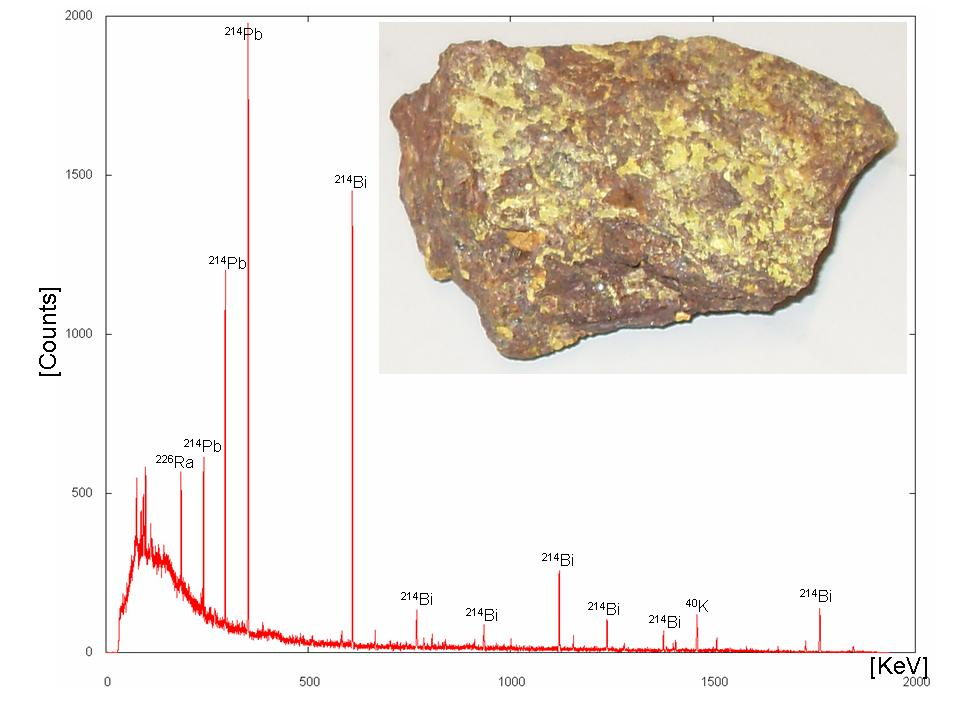
\includegraphics[width = .5\textwidth ,keepaspectratio,frame]{spec.jpg}
\caption{ The gamma-ray spectrum of natural uranium, showing about a dozen discrete lines superimposed on a smooth continuum, \\
allows one to identify the nuclides of the uranium decay chain.\cite{WS}}
\end{figure}
\begin{figure}[!ht]

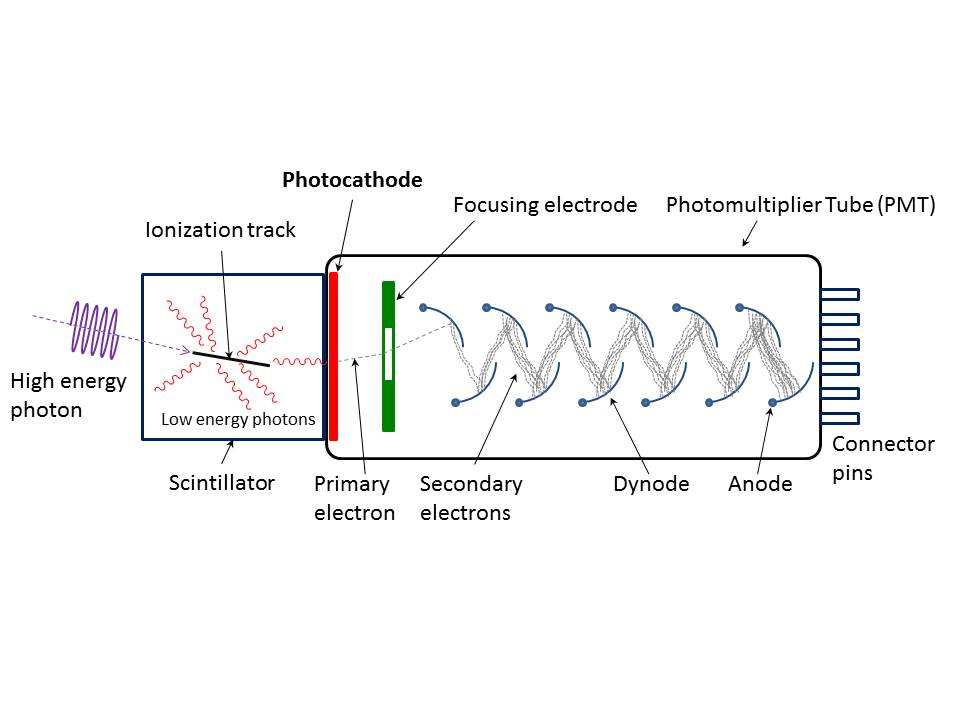
\includegraphics[width = .5\textwidth ,keepaspectratio,frame]{PMT.jpg}
\caption{ Schematic of a photomultiplier tube coupled to a scintillator. This arrangement is for detection of gamma rays.\cite{Sim} The various parts are discussed in further detail in the Theory and methods section of this paper.}

\end{figure}

\section{\label{sec:level1}Introduction}
 The field of Gamma Spectroscopy is the study of the energy spectra of gamma ray sources\cite{WS}. These spectrum allow us to identify various properties of the material that is being analyzed (See Fig. 1 for example). Radioactive elements such as \cs emit gamma ray photons due spontaneous radioactive decay, the process of losing energy in terms of the rest frame of the atomic nucleus. The spectrum of these radioactive sources provide characteristics such as the Back Scatter peaks, Compton Edge, and the radioactive sources known energy. This is all discussed in detail in the following sections. We can further analyze these special characteristics to experimentally verify the mass of the electron. Knowing the mass of the electron allows of to further study it's various properties in details, which are not discussed here.\\

We know that particles follow the energy equation \textit{in free space}:
\[E = pc \quad \rightarrow \quad p = \frac{E}{c} = \frac{\hbar\omega}{c} = \hbar k \]
 Where E is the energy of the gamma photon, p is the gamma photon momentum, and c is the speed of light. This is allows us to find the energy of a \gp from a particular source in some medium.\\ 
\section{\label{sec:level 1}Theory}
We'll use \cs as an example for the following theory,  where\cs is a radioactive isotope of Cesium. Cesium has a total of 78 protons and 78 neutrons, whereas \cs has 55 protons and 82 neutrons. You'll notice a difference of 4 neutrons. This gives \cs it's radioactive properties. \cs has a half life of ~30.17 years and about 95\% decays by beta emission to a \textit{metastable nuclear isomer of barium: $^{137}$barium}\cite{WCS}. The remainder is absorbed into $^{137}$Ba. This is where we observe the emission of $\gamma$ rays. The photon peak of these $\gamma$ rays are 662keV, which is covered in detail later in this paper. Why does this matter? Now that we know some details about this one particular isotope, \cs, we can explore it's uses and how it helps us in determining the mass of the electron.\\
\\

Our approach is to use a Photomultiplier Tube (Fig. 2). The instruments works in a way such that high energy \gp from the \cs source enter the scintillator. When excited by ionizing radiation, the \textit{NaI} crystals in the scintillator absorb the incident \gp energy and re-emit it in the form of light. This light is then sent into the photocathode (red region). When the photocathode is struck by these light photons, it emits electrons due to the photoelectric effect. The electrons now travel to the Photomultipler tube. The electrons are focused towards the electron is accelerated through a voltage potential and becomes incident on the Dynodes where it knocks off more electrons. This is the `multiplied' effect of the electrons where electrons are a multiplied by the process of secondary emission. These secondary emissions are more electrons and the process is repeated a number of times ending in an exponential increase in the final amount of electron emission. This output is run through a pre-amplifier where the signal is converted from current to voltage and various other attributes discussed in the Methods portion of this paper.Finally, the signal is read by a Multi Channel Analyzer that takes readings at specific pulse frequencies (total number of electrons at some energy value) and these are converted into ``channels''. This creates a histogram for spectrum analysis of the data there the histogram channels correspond to the incident energy of the original \gp, as illustrated in Fig. 1.\\

\begin{figure}[ht]
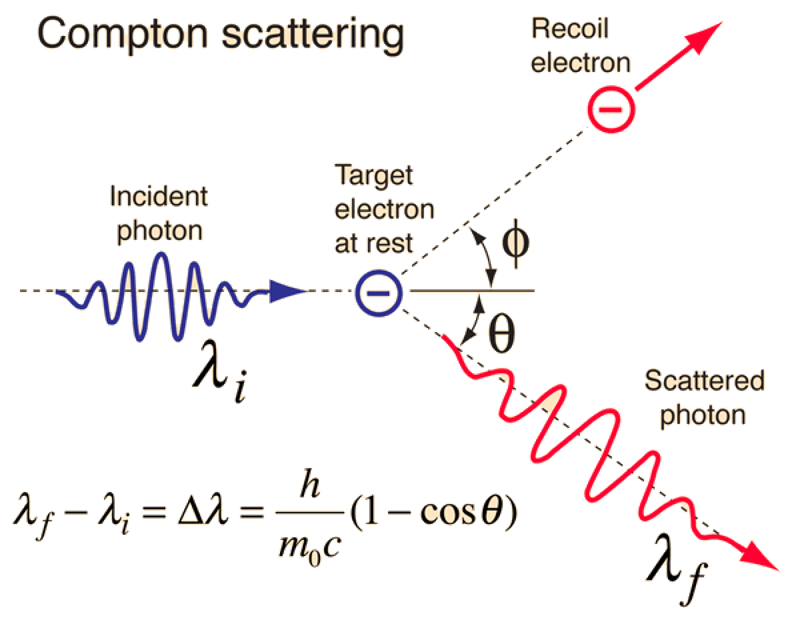
\includegraphics[width = .5\textwidth ,frame]{Compton.png}
\caption{  Compton effect of scattered photons on electrons\cite{HP}. This is a model that illustrates the compton effect of the  light produced by the \textit{NaI} crystals after \gp collision incident on the electron(s) of the thin sheet of the photocathode (see Fig.2).  }
\end{figure}

These components provide an underlying world of physics encapsulated in the data. Compton scattering occurs when the incident photon on the \textit{NaI} crystals hit at varying angles and thus, produces different wavelengths of visible light(Illustarted in Fig. 3) due to conservation of momentum (Fig.3). When the incident \gp are are scattered, they are scattered at varying angles ranging from 0$^{\degree}$ to $180^{\degree}$. We can see this mathematically by the following equations\cite{SBH}, 
\begin{equation}
E_{\gamma}' = \frac{E_{\gamma}}{1 + \frac{E_{\gamma}}{m_0 c^2} (1 - \cos{\theta}) }
\end{equation}
where $E_\gamma$ is the energy of the \gp, $m_0c^2$ is the mass of the electron, and $cos\theta$ is the angle of incidence. We can clearly see that for small angles of $\theta$ (where the \gp hits the \textit{NaI} crystal head on or mostly head on, $cos\theta = 0$. In the data presented later, we can use this equation to find the theoretical backscatter peaks of our sources by assuming that the backscatter peak occures when $\theta$ is maximum (180$\deg$) and thus the equation becomes 
\begin{equation}
E_{\gamma}' = \frac{E_{\gamma}}{1 + 2\frac{E_{\gamma}}{m_0 c^2}}
\end{equation}
and further reduced to
\begin{equation}
\frac{1}{E_{\gamma}'} - \frac{1}{E_{\gamma}} = \frac{2}{m_0 c^2}(1 - \cos{\theta})
\end{equation}
\begin{equation}
\frac{1}{E_{b}} - \frac{1}{E_{\gamma}} = \frac{2}{m_0 c^2}
\end{equation}
where Eq(1) determines the energy of the scattered \gp and Eq(4) is the compton shift in energy for a photon incident with a head on collision such that $\cos{\theta} = 0$.We can immediately see from Eq(3) that the \gp will have maximum energy when no collision occurs which is obvious since there will be no momentum transfer. The \gp will have a minimum energy when a head on collision occurs. This is the backscatter peak. We know from previous experiments that the \textit{Compton shift in energy and wavelength}\cite{DB} is completely dependent on the incident \gp energy. We now know that the backscatter peak will be maximum when the incident photon angle is 180$\degree$ and therefore,
\begin{equation}
E_b = \frac{E_{\gamma}}{ 1 + \frac{2E_{\gamma}}{m_oc^2}}
\end{equation}
and finally we can solve for the rest mass energy of the electron,
\begin{equation}
m_0c^2 = \frac{2}{\frac{1}{E_{\gamma} - \frac{1}{E_{b}}}} = \frac{2E_{b}E_{\gamma}}{E_{\gamma} - E_b}, \text{For Backscatter}
\end{equation}
\begin{equation}
m_0c^2 =2E_{\gamma}\left(\frac{E_{\gamma}}{T_{max}} - 1\right ), \text{For Compton Edge\cite{DB}}
\end{equation}
Where T$_max$ is the energy value of half the height of the Compton edge(Fig. 8) and E$_\gamma$ is the known energy value of the source.






\section{\label{sec:level1}Methods}
We began this experiment by acquiring a few critical components,
\begin{figure}[ht]
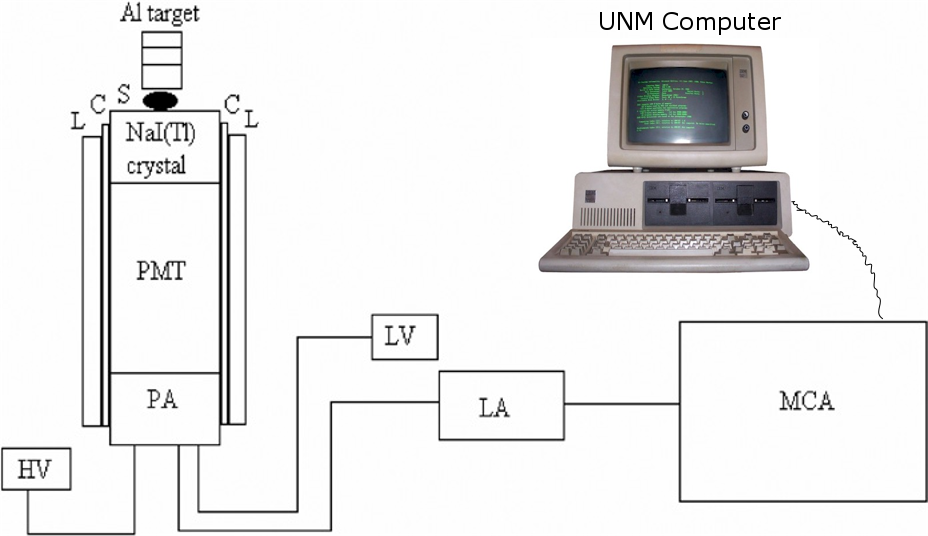
\includegraphics[width = .5\textwidth ]{setup.png}
\caption{ Equipment setup modified from\cite{SBH}. Includes Source(Black Circle), \textit{NaI} Scintillator, Photomultiplier Tube(PMT), Pre-amp(PA), Voltage Source(HV), Multichannel Analyzer(MCA) and the Computer used to run the UCS-30 software.}
\end{figure}
\begin{itemize}
\item Source(s): \cs,\ba,\na,and \co
\end{itemize}
followed by
\begin{itemize}
\item \textit{NaI} Scintillator detector
\item Photomultiplier Tube 
\item Multichannel Analyzer 
\item Voltage source
\item UCS-30 Software
\item Lead `bricks' for housing the Scintillator and source
\end{itemize}

\begin{figure*}[ht]
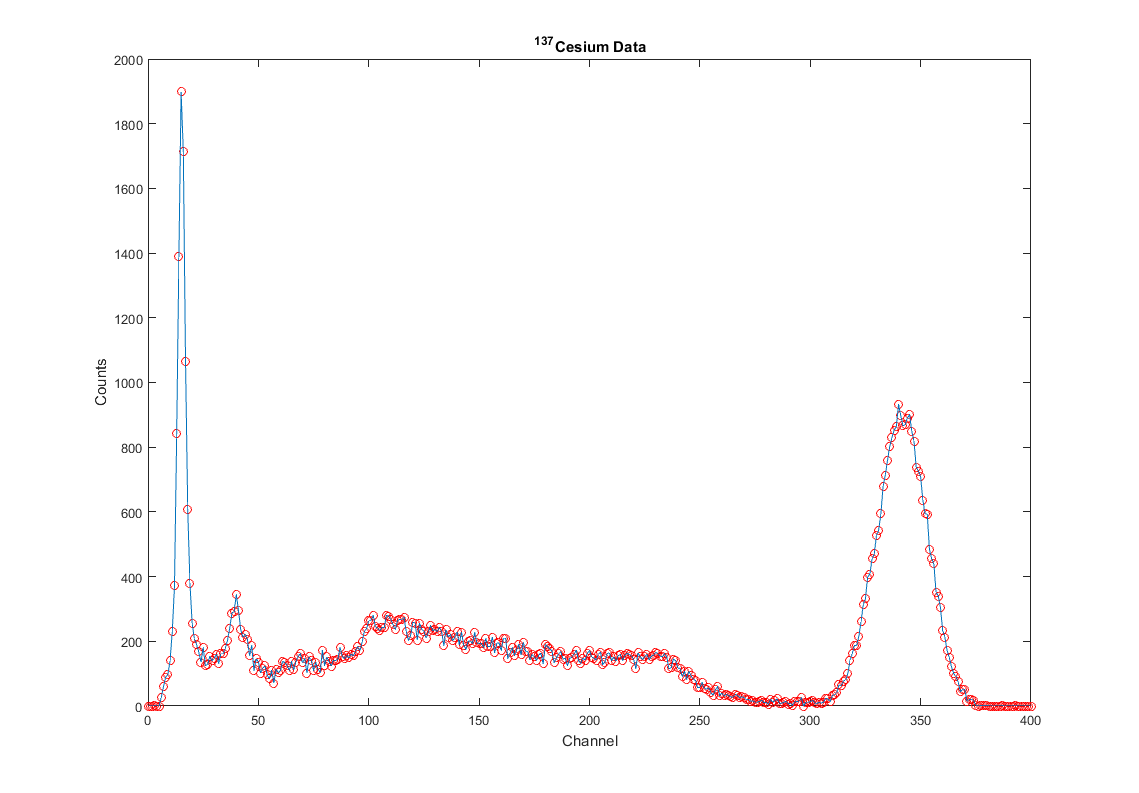
\includegraphics[width =\textwidth ,keepaspectratio,frame]{cs.png}
\caption{Spectrum results for \cs from UPC-30 Software. Generated by Matlab. Channel is the channel that read the energy value of the incident electrons. Counts is the total number of pulses( electrons ) at that energy value. This is a histogram representation and has not been converted to energy values.}
\end{figure*}





The various sources emit \gp radiation. The \gp interact with the \textit{NaI} crystals of the \textit{NaI} Scintillator, where this energy interaction is converted to visible light by the crystals. This light then becomes incident on a thin metal foil called a photo-cathode. The photo-cathode ejects electrons due to the  photo electric effect\cite{WPEE}. The electron is now traveling through the Photomultiplier tube where there is some voltage applied to each of the metal `cups'. The electron is accelerated through this voltage and it becomes incident on the cup which knocks off more electrons. This happens for each subsequent cup and results in a large number of electrons more at the end of the photomultiplier tube. At this stage, the MCA has a specified number of `channels' where it counts the number of electrons (pulses) that hit that channel. These channels produce the spectrum for analysis.\\

We fine tune the resulting spectrum by adjusting various parameters in the UCS-30 software. We  adjust the Gain and the Fine gain. This adjusts the span that the MCA reads. A higher Gain means a smaller area of the channel analyzer is reading some particular energy. The gain configuration we used is a Gain of 2, Fine Gain of 11. The next parameter is the Channel size. We used 1024 Channels, meaning, there are 1024 channels that have discrete energy values associated with them. Lastly, we can control the voltage supplied to the photomultiplier tube. We used the maximum allowed voltage (1200 Volts). Changing the voltage changes the amount of electrons that are produced in the photomultiplier tube. a higher value associated with a higher electron count at the detector. This is because you're accelerating the electron through this voltage potential and hitting the multiplier `cups' with a larger energy. Depending on the experiment, these settings  adjust the resulting spectrum that can now be used for calibration of the source.\\

After we set up all the equipment we begin the experiment. We start with a single source and put it inside the lead brick housing with the \textit{NaI} Scintillator detector. Since the radioactive decay is spontaneous, the detector will pick up signals immediately. Once we have the spectrum, we begin calibration.\\

We know the energies of the sources so this makes calibration easy. We look for the expected energy value of the radioactive source (as seen in Fig. 5 for \cs). We know the channels of the software are representative of energy, so, we expect a peak a certain range (662 MeV for \cs). We can attribute this peak to a channel. That channel is now defined as the energy of the peak (Channel ~348 in Fig. 5 which is roughly equivalent to .662 MeV for \cs). We do this for each of our sources under strict timed conditions, 5 minutes for each source. We also ensure that our parameter settings are not changed between experiment (leaving the gain/voltage the same). When all spectrum have been calibrated, we can quickly verify that we get the expected results. We do this by performing a linear least squares fit of the data (Fig. 6) using the formula in equations below in methods. This experimentally verify what we expect between the various given energies of the sources.

\begin{figure}[ht]
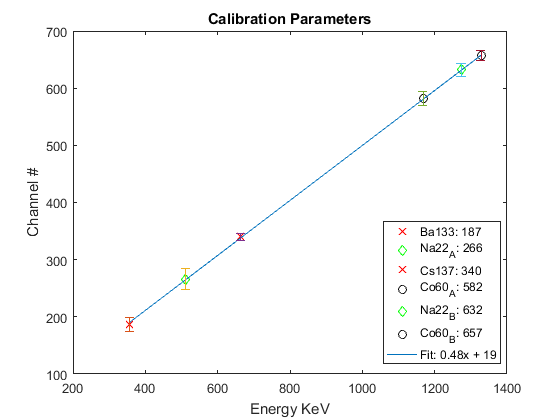
\includegraphics[width = .5\textwidth ,keepaspectratio,frame]{calibration.png}
\caption{ Calibration Fit from Eqn 10 \& 11. Generated by Matlab. Using equations 10 and 11 we generate a linear fit to the channel values of our energy sources and it's corresponding energy value. We get a linear model with slope of .48}
\end{figure}

\begin{figure}[ht!]
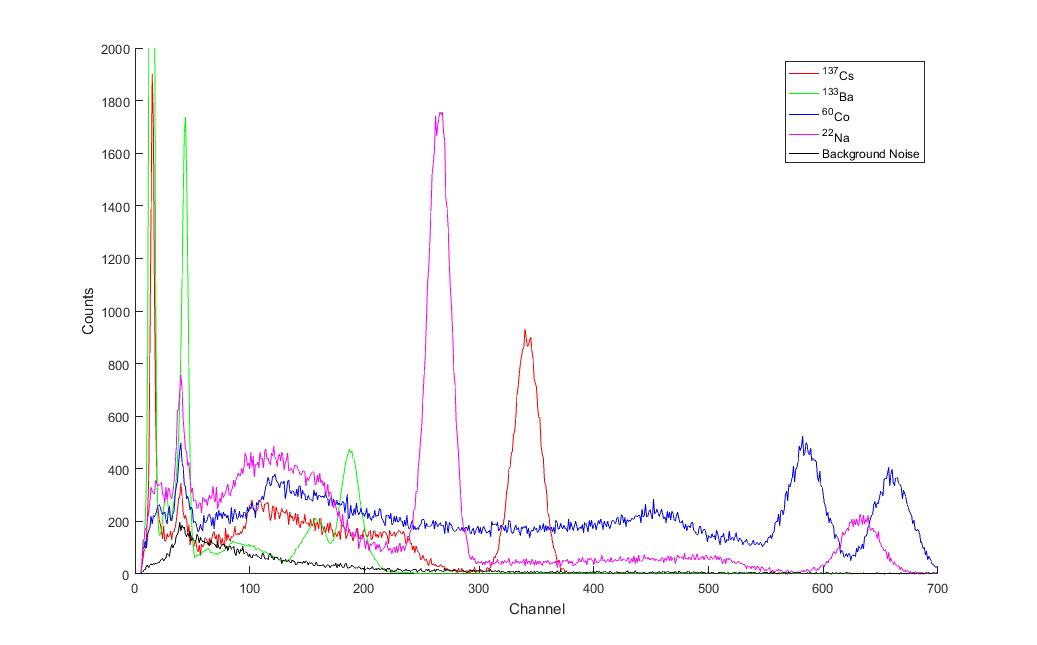
\includegraphics[width = .5\textwidth ,keepaspectratio,frame]{all.png}
\caption{  Spectrum results for all sources ( without noise reduction). Generated by Matlab. We can see the relationship between all the used sources in a more clear picture that helps us to see the linear relationship between the Channel and some corresponding energy value.}
\end{figure}

To show in a more visual manner that these calibrations are consistent with the expected results, we've plotted all the spectrums together (Fig. 7) where you can see that the channels are exactly where we expect them to be if each channel is linearly attributed to an energy. For example, we can see the \cs peak around channel 470 which would be equivalent to .662 MeV, and we can see the two peaks of \co around  Channels ~580 and ~660 respectively, which is equivalent to 1.17 MeV and 1.33 MeV respectively. It follows that the energy data being collected is linear as expected according to a specific channel. The actual channel values would, of course, be different depending on your initial Gain/Voltage/Amp parameters but you would still end up with a linear relationship between channel and energy.

Once our calibration results are verified with the values we expect, we can delve into the various properties. The most important property we want to look at is the Back Scatter peak and Compton Edges of each of our sources individually. These characteristics of the spectrum allow us to find a value for the mass of the electron.

\newpage
\section{\label{sec:level1}Data and Analysis}
\begin{figure*}
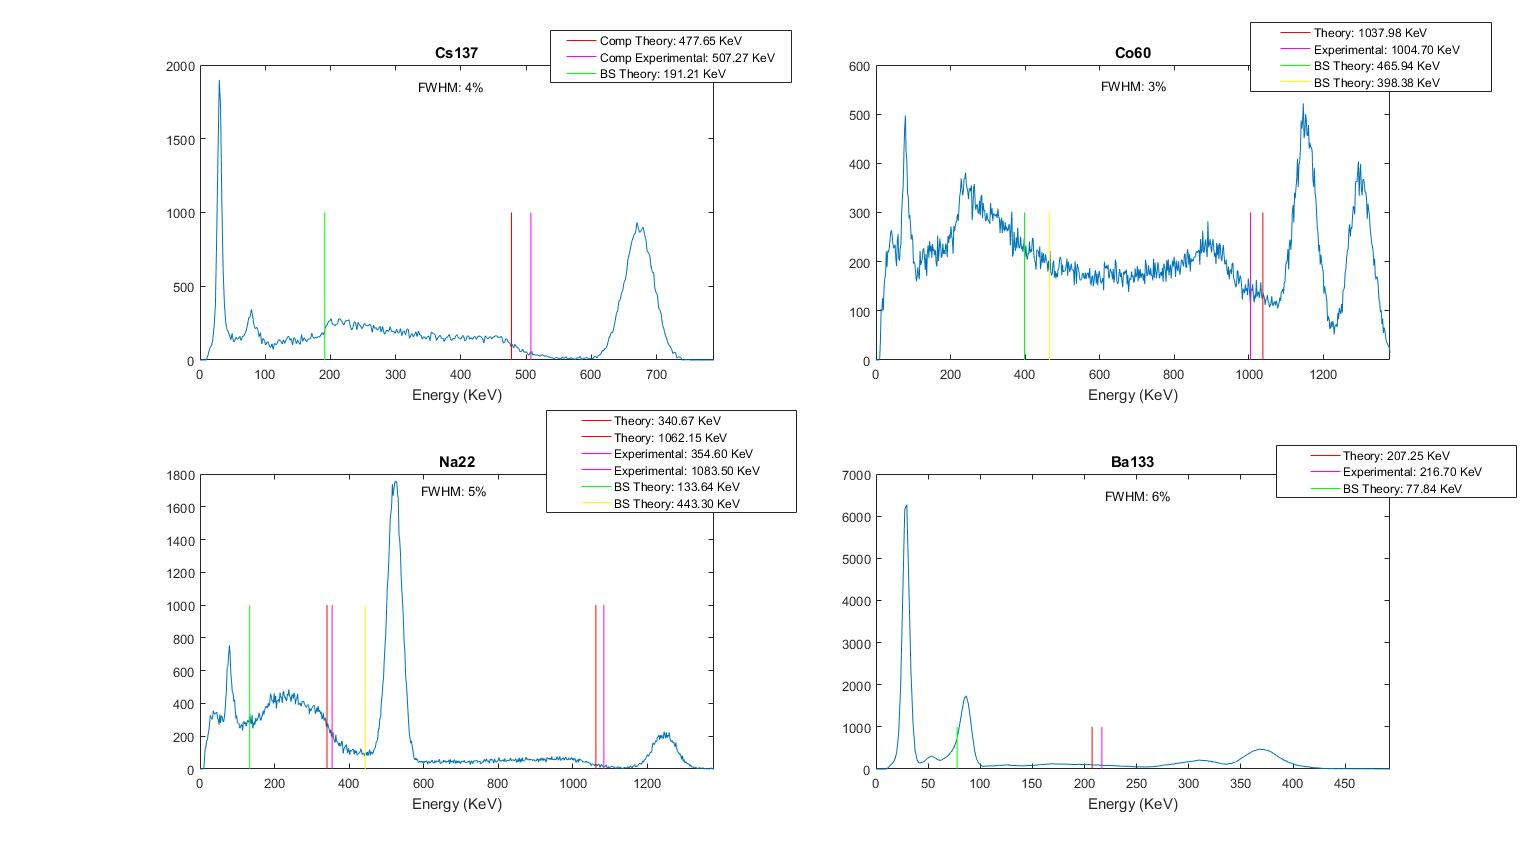
\includegraphics[width = \textwidth ,frame]{ce.jpg}
\caption{  Spectrum cropped to fit only the regions of interest. Generated by Matlab. This shows the 4 sources used as well as their theoretical Compton Edge Values and Theoretical Backscatter Peak values, as well as the experimental values we calculated. Also shown is the Full width half maximum value calculated for each spectrum.}
\end{figure*}
 
 \begin{figure*}[hb]
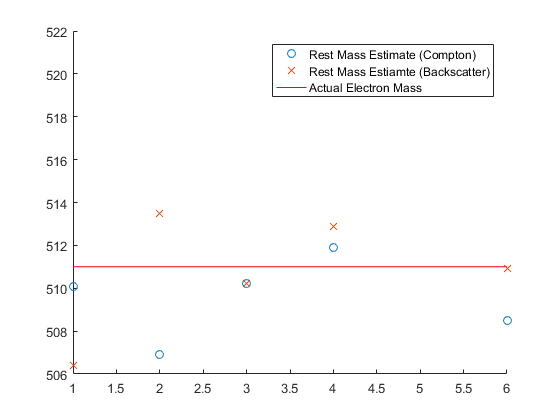
\includegraphics[width = .5\textwidth ,keepaspectratio,frame]{mass.png}
\caption{  Electron rest mass calculated from Compton Edge and Backscatter peaks (labeled accordingly). The x values are merely the total number of masses calculated, 6 in total (one for \cs and \ba, 2 for \na and \co). The y values are the calculated energies and the red line is the known rest mass of the electron.}
\end{figure*}
To begin the Data Analysis, we first remove the noise data (Fig 7) from the gathered data. When the noise is removed from the spectrum data we can identify the Back Scatter peaks and Compton Edges of each source's data. 

We experimentally and theoretically find the expected value of the Compton Edge for each source, Fig 8., where the Compton edge values we used for each source are labeled.  To experimentally find the Compton Edge we use the following equation,
\begin{equation} 
E_{compton} = E \left(1 - \frac{1}{1 + \frac{2E}{m_ec^2}}\right)
\end{equation}
Where $E$ is the energy of the \gp, $m_e$ is the known mass of the electron, and c is the speed of light. You can see these values in Fig 7, Theory.\\

The Back scatter peak was theoretically calculated by using the following equation,
\begin{equation} 
E_{bs} = \frac{E}{2 + \frac{mc^2}{E}}
\end{equation} 

We can see the theoretical Backscatter peak values in Figure 7, as well as the actual observed values.\\

With this spectrum data we analyze the experimental Backscatter Peaks and Compton edges of each of our sources individually. To find the experimental value of the electron,first, we choose 5 local values in the spectrum data that correspond to the backscatter peak and 5 values that correspond to the Compton edge. We find the expected value of these points using the formula\cite{STD}  
\[
\bar x = \frac{1}{N}\sum_{i=1}^Nx_i
\] where $\bar x$ is the expected value of the points chosen. This ensures that we get a good estimate of the true value since the spectrum data is varied. We also find a standard deviation of these points using the formula\cite{STD}
\[
\sigma = \sqrt{\frac{1}{N-1}\sum_{i=1}^N(\bar x - x_i)^2}
\]
where $\bar x$ is the expected value, $x_i$ arr the individual values chosen from the spectrum data, and $\frac{1}{N-1}$ is the unbiased factor of the total number of data points taken. We get a standard deviations of these points to track any statistical errors.
 Rearranging the previous equations (8) and (9) and rearrange them to be (respectively), we plug the 10 chosen into their respective equations below
\[m_ec^2 = 2E\left(\frac{E}{E_{comp}} - 1\right)
\]
where, again, E is the known energy of the source, E$_{comp}$ are the 5 values we chose for the Compton edge, and $mc^2$ is the experimental value of the mass of the electron.
\[m_ec^2 = E\left(\frac{E}{E_{bs}} - 2\right)
\]



From these equations we find the experimental value of the electron mass to be For the Compton Edge and Backscatter peaks.

\begin{center}
\begin{tabular}{|c|c|c|}
\hline
 &Backscatter Peak&  \\
\hline
Source & Experimental(keV) & Theory (keV)\\ \hline
\cs & 506.4$\pm$ 1.6 & 511 \\ \hline
\co & 513.5$\pm$1.3, 510.2$\pm$2.1 & 511 \\ \hline
\na & 512.9$\pm$1.1, 520.6$\pm$1.2 & 511 \\ \hline
\ba & 510.9$\pm$3.9 & 511 \\ \hline
\end{tabular}
\end{center}

\begin{center}
\begin{tabular}{|c|c|c|}
\hline
 &Compton Edge&  \\
\hline
Source & Experimental(keV) & Theory (keV)\\ \hline
\cs & 510.1$\pm$8.6 & 511 \\ \hline
\co & 509.9$\pm$10.8, 510.2$\pm$11.9 & 511 \\ \hline
\na & 511.9$\pm$9.2, 520.6$\pm$4.3 & 511 \\ \hline
\ba & 508.5$\pm$2.8 & 511 \\ \hline
\end{tabular}
\end{center}



Lastly, we find the Full Width Half Maximum of our spectrum data. This allows us to interpret the amount of error we may expect in our data. We get the FWHM by taking the peak energy of the spectrum for each radioactive source. We measure the height of the parabolic peak and talk half of that value. Where this half point value is on the parabola, we take the width value. This width gives us the FWHM value of the data. To convert it to a percentage we take the FWHM and divide it by the expected peak energy of the source. These values are indicated on Fig. 7 for each source.



\section{\label{sec:level1}Conclusions}
From our results it's clear that we get a better estimated value of the electron mass when determine it from the Compton Edge. However, this cannot always be done, for instance, in the case of \co, it may not be immediately obvious where the Compton edge is for either photopeak and may be too difficult to resolve by the observer. We can also see that although we get a better estimate for the Mass of the Electron using the Compton Edge, we also have a higher standard deviation compared to the Backscatter peak method. Upon further analysis we found that the majority of the error in the data is due to statistical error. This is because the the equipment has a finite limit to the amount of energy and resolution of energy that it delineate from. We can see this from the FWHM calculation where the resolution is about 4\% for each of our sources, this accumulates a 4\% in error through all the data. If we account for this resolution error and the statistical errors calculated above, it's clear that the statistical error dominates our experiment. This is of course assuming that all parameters of the UCS-30 software were held constant between runs, the lead bricks were `sealing' the source and \textit{NaI} Scintillator, and the experimental runs were all timed the same.

\section{\label{sec:level5}Bibliography}
\begin{thebibliography}{50}
\bibitem{SBH}
S B Hosur and N M Badger,
\textit{Compton shift in energy and wavelength—a laboratory experiment
}. Am. J. Phys. 55 175\\
\bibitem{STD} Keith Rudick, 
\textit{Statistical Treatment of Data.}
\url{http://spa-mxpweb.spa.umn.edu/resources/MXPStats.pdf}
Spring 2001.\\
\bibitem{PWD}Roger Bach, Damian Pope, Sy-Hwang Liou, and Herman Taeelaan, \textit{Controlled double-slit electron diffraction},  \url{http://iopscience.iop.org/article/10.1088/1367-2630/15/3/033018}\\
\bibitem{DB} Raji Heyrovska, \textit{Compton shift and de Broglie frequency}, Czech Republic, Dolejskova 3, 182 23 Prague 8, Czech Republic.  \url{https://arxiv.org/ftp/physics/papers/0401/0401048.pdf}
\bibitem{ECS} Shanni R. Prutchi and David Prutchi, Ph.D,\textit{Exploring Compton Scattering using the spectrum techniques UCS-20 Universal Spectrometer},\url{http://www.diyphysics.com/wp-content/uploads/2012/01/Compton-Scattering-Experiment-by-Prutchi.pdf}
\bibitem{WCS}\url{https://en.wikipedia.org/wiki/Caesium-137}
\bibitem{HP}\url{http://hyperphysics.phy-astr.gsu.edu/hbase/quantum/compton.html}
\bibitem{WS}  \url{https://en.wikipedia.org/wiki/Gamma_spectroscopy}\\
\bibitem{B}\url{ https://en.wikipedia.org/wiki/Backscatter}\\
\bibitem{S} \url{http://www.ntanet.net/how-\\do-sodium-iodide-scintillation-detectors-work}\\
\bibitem{UCS} \url{http://www.spectrumtechniques.com/wp-content/uploads/2016/12/UCS30-Manual.pdf}\\
\bibitem{Sim} Qwerty123uiop, \url{https://commons.wikimedia.org/w/index.php?curid=29945197}\\
\bibitem{WPEE} \url{https://en.wikipedia.org/wiki/Photoelectric_effect}\\
\bibitem{CE} \url{https://en.wikipedia.org/wiki/Compton_edge}\\
\end{thebibliography}

\end{document}
%
% ****** End of file apssamp.tex ******
